\documentclass[12pt]{article}
\usepackage{a4wide}
\usepackage{graphicx}
\usepackage{mathtools}
\usepackage{placeins}
\usepackage{parskip}
%\usepackage{fullpage}
\usepackage{epstopdf}
\usepackage[margin = 1.0in]{geometry}
\usepackage[font=small,labelfont=bf]{caption}
\usepackage{verbatim}

\usepackage[toc]{appendix}

\usepackage{listings,xcolor}
\usepackage[nottoc]{tocbibind}

\lstset{language=Java}
\lstset{basicstyle={\sffamily\footnotesize},
  numbers=left,
  numberstyle=\tiny\color{gray},
  numbersep=5pt,
  breaklines=true,
  captionpos={t},
  frame={lines},
  rulecolor=\color{black},
  framerule=0.5pt,
  columns=flexible,
  tabsize=2
}

\begin{document}

\pagenumbering{gobble}

\begin{minipage}[b]{110mm}
        {\Huge\bf School of Physics\\ and Astronomy
        \vspace*{17mm}}
\end{minipage}
\hfill
\begin{minipage}[t]{40mm}               
        \makebox[40mm]{
        
\includegraphics[width=40mm]{crest.eps}}
\end{minipage}

\vspace*{2cm}
\begin{center}
        \Large\bf \Large\bf MPhys Project\\
        \LARGE\bf Statistical Physics of Replication Dynamics
\end{center}
\vspace*{0.5cm}
\begin{center}
        Alistair Jones\\  
        {\bf Supervisor:} Dr. R. A. Blythe \\          
        March 2015     
\end{center}

\begin{center}
\subsection*{Abstract}
\end{center}

\newpage
\tableofcontents

\newpage
\pagenumbering{arabic}

\section{Introduction}


\newpage
\section{Background, motivation and aims}
This project investigated the behaviour of language in speech communities. When members of a community, or \emph{speakers}, interact there are numerous possible linguistic objects, e.g. words, phrases or idioms, which can be used to express particular meanings. In many cases there may exist multiple linguistic objects with the same meaning. For example, `couch', `sofa' and `chesterfield' are all words that refer to the same physical object. These linguistic objects are known as \emph{variants}, while the meanings themselves are called \emph{linguistic variables}. In the previous example, the words `couch', `sofa', etc. are the variants and the physical object they correspond to is the linguistic variable. When a speaker wants to express a certain meaning they often must make a choice as to which variant they will use out of a number of alternatives. The focus of this study was on exploring how such choices are made and, more specifically, how preferences towards particular expressions emerge based on interactions between individuals.  

\subsection{History of language change}
For the purposes of this study, there are three key empirical features of historical language change that have been previously established. These features, explained in more detail below, are: the rapid rate of change of new-dialect formation \cite{ref1}; that new conventions spread through the community following an S-curve trajectory \cite{Scurve}; and that the time-scales over which language conventions remain stable are highly diverse \cite{ref3}. The term \emph{new-dialect} simply refers to a way of expressing a certain meaning, i.e.\ a variant, that has not been used in the community before, while a \emph{convention} is a variant used with high frequency among the community. The meaning of the term 'S-curve trajectory' will be explained in the following.

Figure \ref{sofa} shows data from a study into the usage of the words in the above example, namely `sofa', `chesterfield', `couch', `davenport' and `setee', in Canadian English. This was an apparent-time study, meaning data was collected from speakers of different ages, with older speakers taken to be representative of the typical behaviours at appropriate points in the past. Plotting the data in reverse age order thus gives an estimate of the actual change in usage frequency over time, as the 85 year old speakers represent roughly 90 years in the past and so on. 
The key observation is the shape of the curves for `couch' and `chesterfield'. Notice that the usage frequency of `chesterfield' is much greater among 85 year old speakers ($>70\%$) than 10 year old speakers ($<10\% $) while the converse true for `couch', where the minority of 85 year old speakers ($<10\% $) and the vast majority of 10 year old speakers ($\approx 90\%$) are users. In other words, over time the convention changes from `chesterfield' to `couch'. The former is thus referred to as the \emph{outgoing variant} while the latter is the \emph{incoming variant}. Figure \ref{sofa} provides an example of the result stated previously, that conventions change according to an \emph{S-curve trajectory}: the rate of growth initially accelerates until both the incoming and the outgoing variant are widely used, after which the rate of growth decelerates as the incoming variant becomes used by the majority of speakers \cite{Scurve}.\\
\begin{figure}[h!]
\begin{center}
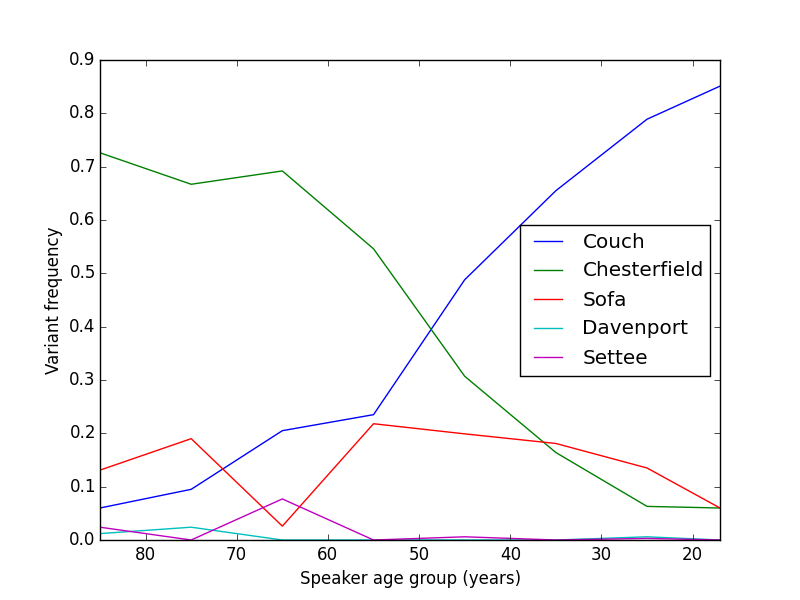
\includegraphics[width=\textwidth]{Scurves.png}
\end{center}
\caption{Variation in usage frequency of different furniture terms in Canadian English. Data collected using an apparent-time study, meaning data collected from speakers of different ages with older speakers taken to be representative of typical behaviour at an appropriate time in the past. Plotting the data in reverse age order thus gives an estimate of the actual change in usage frequency over time. Data originally from \cite{20}.}\label{sofa}
\end{figure}\\
%Question: should I fit to these curves?
An obvious question raised by this plot is: how do S-curves trajectories for conventions occur? The answer, which is discussed in the 'Previous Results' section, helps form the foundations of this investigation. As a brief aside, it might be interesting to ask: why is it `couch' that succeeds in becoming the convention and not one of the other variants? The graph seemingly provides no reason for the emergence of `couch' as the preference. However, while this is clearly very closely related to the focus of this investigation, answering this question did not form part of this project.

%The rapid rate of change of new-dialect formation paragraph \cite{ref1}. 



\subsection{Selection mechanisms}
Language change can be modelled as a two-step evolutionary operation, consisting of the generation of variants and the propagation of these through the speech community \cite{croft}. The fundamental dynamical process is replication, in particular the replication of linguistic objects and structures, or variants, through speech. Speaking a collection of variants is referred to in the following as producing an \emph{utterance}. Each time a speaker produces an utterance he/she replicates variants they have heard before. In other words, this replication process is controlled by the speaker and their knowledge of the language, which has been previously determined by the language he/she has been exposed to. The interactions a particular speaker has experienced in the past will therefore influence those in the future, i.e.\ a speaker builds a usage-based memory of the variants which controls the outcome of future interactions. 

The central element in processes of the type above is unit of replication, called the \emph{replicator} \cite{hull}. An example of a replicator in biological evolution would be a gene, which is replicated during the production of sex cells (meiosis) and passed on to the offspring of an individual. In language change the replicator is a variant, which is replicated during speech interactions between individuals \cite{lc&v}.\ \emph{Selection} is the process which determines the frequencies with which different replicators are replicated. In general it can be argued that \emph{interactors} are also required for selection to occur \cite{hull}. Returning to the example of biological evolution, the interactors are organisms which are responsible for replication through interactions between one another. In other words, an organism reproducing means that it's genes are replicated and are thus propagated throughout a population, otherwise the genes will become extinct. Similarly, in language change the speakers are the interactors which replicate certain variants; if speakers select to replicate one variant more than another then the unused variant will eventually become extinct. Figure \ref{repInt} provides an illustration of replicators and interactors in the context of linguistic theory. Note the subtle difference between these two systems: in biology a replicator (a gene) "belongs to" an interactor (an organism) and the survival of a replicator is due to the "fitness" of the interactor; in linguistic theory however, there is not a one-to-one relationship between a replicator (a variant) and the interactor (the speaker who produces it) and the replicator's survivability arises from the social standing of individuals using that variant.

\begin{figure}[h]
\begin{center}
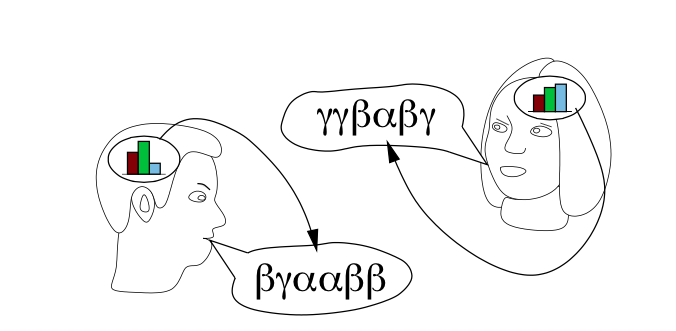
\includegraphics[width=\textwidth*8/10]{replicatorsInteractors.png}
\end{center}
\caption{Speakers (interactors) produce utterances of the variants (replicators) $\alpha$, $\beta$ and $\gamma$ of some linguistic variable, according to their individual usage based memories of those variants \cite{USM}.}\label{repInt}
\end{figure}

The theory of utterance selection distinguishes between two forms of selection: \emph{interactor selection} and \emph{replicator selection} \cite{croft}. Interactor selection labels the fact that an interactor may be influenced by some interactors more than others. The difference in influence can be due to either the frequency with which certain interactors interact, i.e.\ the more often two individuals interact the greater their influence on one another, or the interaction of an interactor with a particularly strongly influential individual. The former can be thought of, in context of language behaviour, as an individual interacting with their neighbour more than with someone from another town, while an example of the latter would be the influence over an individual a friend has in contrast to an acquaintance. Replicator selection stems from the replicator and corresponds to the preference of an interactor towards a particular replicator. Replicator selection is thus an intrinsic property of a replicator. In a speech community, an example may be when a speaker prefers to use words or phrases commonly used by speakers they wish to associate with. 

In summary: variants of linguistic variables and speakers correspond to replicators and interactors respectively with interactions propagating replicators through the community; during speech a speaker utters a collection of variants which are replicated; variants are selected according a speaker's usage-based knowledge of the language, which arises as a consequence of the two sources of selection discussed above; the action of selection during each interaction alters a speakers knowledge of the language and thus influences the frequencies with which certain variants will be replicated in future; consequently it is possible for a variant to out-compete others, i.e. for the community to collectively reach a consensus as to which variant they use.

\subsection{Previous studies}
The theory of utterance selection can be used to define a model known as the `Utterance Selection Model' (USM), a detailed description of which is given in the Method section below. The following presents a brief summary of some of the behaviour that has previously been established for the USM. 

A fundamental feature of the USM is that speakers monitor their own utterances in addition to the speech of others. In other words the utterances of a speaker partly influences their own usage frequencies. This allows for some interesting observations even within single-speaker systems, as a speaker's own utterances will cause fluctuations in their variant frequencies. In particular these fluctuations eventually ensure the usage frequencies reach \emph{fixation} \cite{USM}, which is a state where only one variant is ever spoken. This result can be thought of in a similar way to the example of biological evolution above, in the sense that one replicator goes extinct while another flourishes. Note that this result was obtained without replicator selection, i.e.\ with interactor selection operating only. 

There are two types of multi-speaker models: those in a `flat' society and those on a network. A flat society is one in which all speakers interact equally often and are influenced the same amount by the utterances of every other speaker. A network of speakers is a more complex system in which neither of these statements are true. First consider the flat society. As in the single-speaker model, fluctuations in variant frequencies occur until one of the variants reaches fixation (i.e.\ is the only one remaining) \cite{USM}. In particular, the number of interactions for fixation to occur was found to be proportional to the number of speakers squared. As this investigation considered interaction to happen in parallel, this corresponds to the time to fixation increasing linearly with the number of speakers (because every speaker interacting each time step cancels the square in the number of interactions). 
%
%%%%%%%%%%%%%%%% Question: should I put a physical example of a flat society and a complex network?

Return now and consider the more general case of a complex network of speakers, where speakers do not interact equally often and speakers have varying levels of influence over one another. Such networks comprise speakers located at different sites, or \emph{nodes}, with links between them allowing for interactions between those speakers. Interestingly it can be shown that the network structure has a dramatic effect on the likelihood a low-frequency variant goes to fixation, and the time it does to do so \cite{ref12}. In particular, in the case where the variance in the number of neighbours of each node diverges for infinitely large networks, the number of interactions for fixation can be much faster ($O(N)$) than in a flat society ($O(N^2)$). This does however rely on large asymmetries between the affect that two speakers have on each other, i.e.\ the utterances of speaker 1 must affect speaker 2 much greater/less than those of speaker 2 influence speaker 1. These asymmetries typically arise through large differences between the number of neighbours any two nodes have, although it is possible to construct a more uniform network and vary the level of influence a single interaction between two speakers has over each of their frequencies to similar effect \cite{ref15}. Furthermore, if the influence an interaction has over two speakers is the same for all speakers then the fixation times independent of the network structure, provided the nodes are sufficiently well connected \cite{ref12}. 

Finally, and most importantly for this investigation, in models that only invoke interactor selection, and not replicator selection, conventions have been found to typically follow a trajectory given by the exponential function, $x(t) = 1 − e^{−kt}$ for some k ****citation needed****. This is not consistent with the S-shape characteristic of historical language change as discussed above, which follows a trajectory given by the logistic function, $x(t) = \frac{1}{1 + e^{a(t-t_0)}}$ for constants $a$ and $t_0$ \cite{ref2}. 

\subsection{Emergence of replicator selection}
Recall that interactor selection is due to individuals being affected by the utterances of some speakers more than others, while replicator selection is selection due to an intrinsic preference of a speaker towards a particular variant. Although interactor selection is relatively intuitive in the context of physical systems, e.g.\ one can picture a scenario in which a person will interact with some people more than others, the physical origin of replicator selection is not as clear. What is clear is that earlier studies, as detailed above, indicate that replicator selection is an essential component in obtaining the S-shape characteristic of historical language change. However, whenever replicator selection has been included it is been pre-specified from the outset, i.e.\ each speaker has given a fixed, pre-determined boost in preference towards a particular variant. What is unclear is how these shared preferences emerge from interactions between speakers. The hypothesis of this investigation was that emergence of replicator selection could be achieved by exploiting existence of interactor selection. How this was achieved is explained in the Method section. The aim of this project, once a mechanism for this emergence had been established, was to explore the resulting effects and phenomena on two slightly different types of speech communities, which are discussed below.

\newpage
\section{Method}


\subsection{Stochastic modelling}
As stated above, the two sources of selection involved in the model presented were interactor and replicator selection. The former is associated to both how often a particular variant is heard by a speaker and how strongly influenced by others a speaker is, while the latter incorporates the intrinsic preference of a speaker towards a particular variant. The Utterance Selection Model (USM) mentioned above formed the basis for the model used in this investigation. In order to include replicator selection, a refinement of the original USM, which is presented in \cite{refined}, was used. While interactor selection is present in both models, the refined USM extends the original by adding replicator selection
\subsubsection{Refined utterance selection model}
This model comprises $N$ speakers and a single linguistic variable with a set of $V$ variants, where each speaker has knowledge of all variants. Speakers and variants are indexed by $i$ and $v$ respectively, with $i \in \{1, 2, ... , N\}$ and $v \in \{1, 2, ..., V\}$. The probability of speaker $i$ speaking variant $v$ is $x_{iv}$, which gives the frequency with which the speaker perceives the variant to be used in the community. In this and subsequent models, speaking is the production of one or more tokens, each corresponding to an instance of a particular variant. The number of tokens of variant $v$ produced by speaker $i$ is $n_{iv}$. The probabilities $\{x_{iv}\}$ are modified by the interactions between different speakers in the community. The interaction process is as follows: 
\begin{itemize}
\item[1.] Two speakers, $i$ and $j$, are chosen at random to interact.
\item[2.] Both generate a set of $T$ tokens, with $\sum\limits_{v = 1}^{V} (n_{iv} + n_{jv}) = T$. 
\item[3.] Both then construct a collection of \emph{perceived frequencies}, $y_{iv}$ and $y_{jv}$, which represent each speakers perception of the use of each variant (by both speakers). For speaker $i$ this is given by
\begin{equation} \label{y}
y_{iv} = f_{iv}\left(\frac{n_{iv}}{T}\right) + H_{ij}f_{iv}\left(\frac{n_{jv}}{T}\right)
\end{equation}
where $H_{ij}$ gives the weight speaker $i$ ascribes to the utterances of speaker $j$ and the function $f_{iv}$ is defined below. The weight parameter $H_{ij}$ represents the preference speaker $i$ has towards speaker $j$ where, for example, $H_{12}>H_{13}$ means speaker $2$ has a greater influence over the speech of speaker $1$ than speaker $3$ has. The weights therefore provide the mechanism by which interactor selection is incorporated into the model. There is an analogous expression for speaker $j$. 
\item[4.] Each speaker modifies their speech behaviour via
\begin{equation}\label{x}
x_{iv}' = \frac{x_{iv} + \lambda y_{iv}}{Z}
\end{equation}
where $\lambda$ is a small parameter ($\lambda \approx 0.01$) controlling the amount each interaction affects a speakers behaviour and $Z = 1 + \lambda \sum\limits_{v} y_{iv} = 1 + \lambda (1 + H_{ij})$, which is found by enforcing that $\sum\limits_{v} x_{iv}' = 1$ and where the last equality holds for $f_{iv}(u) = u$ in \eqref{y}. Again there are analogous expressions for speaker $j$.
\end{itemize}
An important point to note in the above is that the weights $H_{ij}$ are not necessarily symmetric, i.e.\ it is possible to have $H_{ij} \neq  H_{ji}$ which is the case if speaker $i$ does not pay as much attention to speaker $j$ as $j$ does to $i$ or visa versa. However for the purposes of this study the weights are all symmetric. 

The function $f_{iv}(u)$ allows for a number of effects to be included; most importantly replicator selection. The intrinsic replicator weight speaker $i$ ascribes to variant $v$ is given by $S_{iv}$, which can then be incorporated into the form of $f_{iv}$. For this investigation $f_{iv}$ was defined to be
\begin{equation}\label{f}
f_{iv}(u) = \min \left\lbrace 1, (1 + S_{iv})u \right\rbrace
\end{equation}
which ensures that variants with a higher $S_{iv}$ will be preferred. The minimum value of $1$ and $(1 + S_{iv})u$ is chosen as it ensures that $y_{iv}$ satisfies
\begin{equation}
y_{iv} \leq 1 + H_{ij}
\end{equation}
which is required for $Z \approx 1 + \lambda (1 + H_{ij})$, as is the case for $f_{iv}(u) = u$. This normalisation is very useful for performing computations, as a relatively large amount of calculations can be avoided.   

\subsubsection{Emergence of replicator selection}
As stated previously, the main aim of this investigation was to study the emergence of replicator selection from interactions between the speakers; in particular by exploiting the pre-existing variation in the interactor weights. Replicator selection enters in through the intrinsic replicator weight speaker $i$ ascribes to variant $v$, $S_{iv}$, which changes according to interactions between speakers in a similar way to the variant frequency $x_{iv}$. To construct the replicator weights the model used here gives speakers the ability to record the behaviour of specific individuals through the definition of a set of variables $\{u_{ijv}\}$, which is the frequency that speaker $i$ perceives speaker $j$ to use variant $v$. The replicator weights are then taken to be given by
\begin{equation}
S_{iv} = \sigma \sum\limits_{j} H_{ij}u_{ijv}
\end{equation}
where $\sigma$ is an independent parameter. Note that when $\sigma = 0 $, $S_{iv} = 0$ and thus $f_{iv}(u) = u$ is recovered in (\ref{f}), which is the case when there is no replicator selection as in the original USM. The form for $S_{iv}$ is such that if a speaker $j$ uses a particular variant with a high frequency, and $i$ ascribes a high interaction weight, $H_{ij}$, to the utterances of $j$, then $S_{iv}$ will be large in comparison to the replicator weight of other variants. The update rule for $u_{ijv}$ is
\begin{equation}\label{u}
u_{ijv}' = \frac{u_{ijv} + \gamma (\frac{n_{jv}}{T})}{1 + \gamma}
\end{equation}
where $\gamma$ is similar to $\lambda$ in the previous section, as it scales the affect of interactions on $u_{ijv}$, and the normalisation $1 + \gamma$ is due to the requirement that $\sum\limits_{v} u_{ijv} = 1$. There is an analogous expression for $u_{jiv}$. This expression can be used to derive an update rule for $S_{iv}$, 
\begin{equation}\label{S}
S_{iv}' = \frac{S_{iv} + \sigma \gamma \sum\limits_{j} H_{ij}(\frac{n_{jv}}{T})}{1 + \gamma}
\end{equation}
which is more useful for performing computations as fewer variables need to be stored. Again a similar expression exists for $S_{jv}$. The new update sequence for the usage frequencies $x_{iv}$ and $x_{jv}$ is then as follows:
\begin{itemize}
\item[1.] Two speakers, $i$ and $j$, are chosen at random to interact as above.
\item[2.] Both generate $T$ tokens according to their corresponding usage frequencies $x_{iv}$ and $x_{jv}$
\item[3.] The replicator weights $S_{iv}$ and $S_{jv}$ are updated according to \eqref{S} and the analogous expression for speaker $j$.
\item[4.] The usage frequencies $x_{iv}$ and $x_{jv}$ are then updated as in the USM, using \eqref{f} and a similar expression for $f_{jv}$.
\end{itemize}
The difference between this model and the original USM is the addition of step 3, in which the replicator weights are updated. When put into the context of an update cycle, it is clear that using \eqref{S} instead of \eqref{u} in step 3 prevents both storing the $u_{ijv}$ values, of which there will be many, and summing expression \eqref{u} over $j$ to obtain $S_{iv}$. This makes the cycle much more tractable with regards to performing computer simulations.

\subsubsection{Two-group model}
\subsubsection{Linear chain model}

\subsection{Mathematical analysis}
Analysing models such as the USM, with a stochastic variable $X$ and the updated variable at the end of a time step $X'$, requires the calculation of quantities known as the \emph{jump moments}, generally given by
\begin{equation}\label{a}
a_k(X) = \left\langle \left(X' - X \right)^k \right\rangle.
\end{equation}

For a stochastic process with a single random variable, the jump moments can be use to derive the following Fokker-Planck equation \cite{fpeqn}:
\begin{equation}\label{fp}
\frac{\partial P (X,t)}{\partial t} = - \frac{\partial}{\partial X} \left[ a_1(X)P(X,t) \right] + \frac{1}{2}\frac{\partial^2}{\partial X^2} \left[ a_2(X)P(X,t) \right]
\end{equation}
The first term in this equation gives the deterministic contribution to the dynamics, while the second term gives the leading stochastic contribution. One could proceed to calculate higher-order stochastic terms although it is not necessary in this study. For a generalised analysis of the Fokker Planck equation, including the extension to more than one variable, see \cite{fpeqn}. Rather than pursuing a full Fokker-Planck equation, this project focussed on using the jump moments to derive a mean field theory for the usage frequencies. In particular, the aim was to find an expression for the change in the usage frequencies and the percieved frequencies with respect to time, $\frac{\mathrm d x_i}{\mathrm d t}$ and $\frac{\mathrm d u_{ij}}{\mathrm d t}$ respectively.

Now consider the USM with replicator selection defined previously and note that the following calculations are kept as general as possible, with specification to the two-group and linear chain cases below. Furthermore consider the case where there are only two variants of a single variable. The probability that a particular pair of speakers, $i$ and $j$, is selected to interact is $G$, the expression for which of course depends on the system. The usage frequencies $x_i$ are thus updated with probability $G$ each time-step, according to 
\begin{equation}\label{x2}
x_i' = \frac{x_i + \lambda y_i}{Z},
\end{equation}
with an analogous expression for $x_j$, and remain unchanged with probability $1-G$. This expression is the same as (\ref{x}) with the $v$ subscripts dropped because there are only two variants, so specifying one frequency specifies the other. In other words, let $x_{i1} = x_{i}$ which means $x_{i2} = 1- x_{i}$, so that $ x_{i1} + x_{i2}=  1$. Recall that $y_i$ is given by
\begin{equation} \label{y2}
y_i = f_i\left(\frac{n_i}{T}\right) + H_{ij}f_i\left(\frac{n_j}{T}\right),
\end{equation}
where it is important to recall that $T$ is the total number of tokens produced during an interaction. The random variable in eq. (\ref{y2}), and thus in (\ref{x2}), is $n_{j}$, which is the number of tokens of variant 1 that speaker $j$ produces in the interaction. The number of tokens of variant 2 produced by speaker $j$ is therefore $T-n_j$, i.e.\ $n_{j1} = n_j$ and $n_{j2} = T - n_{j}$ to give $n_{j1} + n_{j2} = T$.  As there are two variants, i.e.\ two possible outcomes of each utterance, $n_j$ is a binomial random variable. The mean of $n_j$ is thus given by
\begin{equation}\label{mean}
\left\langle n_j \right\rangle = T x_j
\end{equation}
and the variance is
\begin{equation}\label{variance}
\left\langle n_j^2 \right\rangle - \left\langle n_j \right\rangle^2 = T x_j (1 - x_j).
\end{equation}
These quantities will become important momentarily. Before that, writing (\ref{x2}) in a form compatible with (\ref{a}), i.e.\ to write an expression for $x_i' - x_i$, required an explicit expression for the normalisation Z. As a brief notational aside, in the following it is useful to label quantities with a tilde that correspond to the usage of variant 2, e.g.\ $\tilde{x_i} \equiv x_{i2} = 1 - x_i$. For the two-variant case, normalisation is therefore always such that $x_i + \tilde{x_i} = 1$ as above. This, in conjunction with eq. (\ref{x2}), can be used to write
\begin{equation}
Z = x_i + \lambda y_i + \tilde{x_i} + \lambda \tilde{y_i} = 1 + \lambda \left(y_i + \tilde{y_i} \right),
\end{equation}
where $y_i$ and $\tilde{y_i}$ are speaker $i$'s perceptions of the usage of variants 1 and 2 respectively, i.e.\ $y_{i1} = y_i$ and $y_{i2} = \tilde{y_i}$.
Under the assumption that $\lambda$ is small, 
\begin{equation}\label{xminusx}
x_i' - x_i = \lambda \left[ y_i - \left( y_i + \tilde{y_i} \right) x_i \right] + O\left(\lambda ^2 \right).
\end{equation}
In order to find an expression for the RHS, return to eq. (\ref{y2}), with an analogous expression for $\tilde{y_i}$, so that
\begin{equation}
y_i + \tilde{y_i} = f_i\left( \frac{n_i}{T} \right) + H_{ij}f_i\left( \frac{n_j}{T} \right) + \tilde{f_i}\left( 1 - \frac{n_i}{T} \right) + H_{ij}\tilde{f_i}\left(1 - \frac{n_j}{T} \right). \\
\end{equation}
In the case where $f_i(u) = (1 - S_i)u$ and $\tilde{f_i} = (1 - \tilde{S_i})u$, as given in (\ref{f}), this becomes
\begin{equation}\label{yplusy}
y_i + \tilde{y_i} = 1 + H_{ij} + S_i\left( \frac{n_i}{T} + H_{ij}\frac{n_j}{T} \right) + \tilde{S_i}\left( \left[ 1 - \frac{n_i}{T} \right] + H_{ij} \left[ 1 - \frac{n_j}{T}\right]\right).
\end{equation}
Substituting (\ref{yplusy}) into (\ref{xminusx}) therefore gives, 
to leading order in $\lambda$,
\begin{multline}
x_i' - x_i = \lambda \left[ \frac{n_i}{T} - x_i + H_{ij}\left( \frac{n_j}{T} - x_i \right) \right. + S_i(1 - x_i)\left(\frac{n_i}{T} + H_{ij}\frac{n_j}{T} \right) \\ - \left.\tilde{S_i}x_i \left( \left[ 1 - \frac{n_i}{T} \right] + H_{ij} \left[ 1 - \frac{n_j}{T}\right]\right)   \right].
\end{multline}
It is useful to return to the definition of $S_i$ in (\ref{S}), where
\begin{align}
S_{i} = \sigma \sum\limits_{j} H_{ij}u_{ij} & \quad \text{and} \quad \tilde{S_{i}} = \sigma \sum\limits_{j} H_{ij}\tilde{u}_{ij} 
\end{align}
where $u_{ij}$ and $\tilde{u_{ij}}$ are the frequencies that speaker $i$ perceives $j$ to use variants 1 and 2. As $u_{ij} + \tilde{u}_{ij} = 1$, the second term in this expression becomes
\begin{equation}
\tilde{S_i} = \sigma \sum\limits_{j} H_{ij} (1 - u_{ij}) = \sigma \sum\limits_{j} H_{ij} - S_i = S_i^* - S_i,
\end{equation}
where $S_i^* \equiv \sigma \sum\limits_{j} H_{ij}$. Using this result, in addition to the statistics of the binomial distribution as given by (\ref{mean}) and (\ref{variance}), the first jump moment for the usage frequencies, after rearranging, is given by
\begin{multline}
a_1(x_i) = \left\langle x_i' - x_i \right\rangle = \\ G \lambda \left[ H_{ij}(x_j - x_i) + (2S_i - S_i^*)x_i(1-x_i) + S_i H_{ij}(1-x_i)x_j - (S_i^* - S_i)H_{ij}x_i(1-x_j)\right].
\end{multline}
In the original USM, it was conventional to take $H_{ij} = \lambda h_{ij}$, where $h_{ij}$ is typically $O(1)$ so that $H_{ij} \sim \lambda $. ***Reason?***.  This means that the replicator weights $S_i$ and $S_i^*$ will also be of order $\lambda$ and can be rewritten $S_i = \lambda s_i$ and $S_i^* = \lambda s_i^*$, where 
\begin{align}\label{sisistar}
s_{i} = \sigma \sum\limits_{j} h_{ij}u_{ij} & \quad \text{and} \quad s_{i}^* = \sigma \sum\limits_{j} h_{ij}.
\end{align}
Substituting these expressions for the interactor and replicator weights, retaining only terms up to $O(\lambda)$, leads to 
\begin{equation}
a_1(x_i) = G \lambda^2 \left[ h_{ij} (x_j - x_i) + (2s_i - s_i^*)x_i(1-x_i) \right].
\end{equation}
Assuming that fluctuations can be neglected, so that $\left\langle x_i ^2 \right\rangle \approx \left\langle x_i  \right\rangle^2$, the recipe for the time-derivative of the usage frequencies is
%%%%%%%%%%%%Question: where does the sum over i =/= j come from?
\begin{equation}\label{mf1}
\frac{\mathrm d x_i}{\mathrm d t} = \sum\limits_{j \neq i} \left\langle a_1(x_i) \right\rangle = G \lambda^2 \sum\limits_{j \neq i} \left[ h_{ij} (\left\langle x_j \right\rangle -\left\langle x_i\right\rangle) + (2\left\langle s_i \right\rangle- s_i^*)\left\langle x_i\right\rangle(1-\left\langle x_i\right\rangle) \right],
\end{equation}
where $\left\langle s_i^*\right\rangle = s_i^*$, as $s_i^*$ is independent of the frequencies, and 
\begin{equation}
\left\langle s_i \right\rangle = \sigma \sum\limits_{j \neq i} h_{ij} \left\langle u_{ij} \right\rangle
\end{equation}

Calculating the analogous expression to (\ref{mf1}) for $u_{ij}$ is less strenuous. From (\ref{u}), $u_{ij}$ is updated according to
\begin{equation}
u_{ij}' = \frac{u_{ij} + \gamma \frac{n_j}{T}}{1+\gamma},
\end{equation}
where again the random variable is $n_j$ and gamma is a small parameter. Recall that an update occurs with probability $G$ and therefore that no change happens with probability $1-G$. It is convenient to write
\begin{equation}
u_{ij}' - u_{ij} = \gamma \left[ \frac{n_j}{T} - u_{ij}\right] + O\left(\gamma^2 \right).
\end{equation}
Then, retaining only terms up to $O(\gamma)$, 
\begin{equation}
a_1(u_{ij}) = \left\langle \left( u_{ij}' - u_{ij} \right) \right\rangle = G \gamma \left\langle \frac{n_j}{T} - u_{ij} \right\rangle = G \gamma(x_j - u_{ij}) 
\end{equation}
Finally, the time-derivative of $u_{ij}$ is given by
\begin{equation}\label{mf2}
\frac{\mathrm d u_{ij}}{\mathrm d t} = \left\langle a_1 (u_{ij}) \right) = G \gamma ( \left\langle x_j \right\rangle - \left\langle u_{ij} \right\rangle).
\end{equation}
Expressions (\ref{mf1}) and (\ref{mf2}) together form a \emph{mean field theory} for the frequencies. The main purpose of deriving these equation was to find and explore the steady states of the modified USM. The steady states of (\ref{mf1}) were of particular interest. A steady state is one in which the time derivatives are zero. The usefulness of (\ref{mf2}) is found in observing that it implies for a steady state that $x_j = u_{ij}$, which is the case where speaker $i$ has an accurate perception of the utterances of speaker $j$. In the following (\ref{mf1}) is specified to the two cases of interest in this investigation: the two-group and linear chain models.

\subsubsection{Two-group model}
As stated above, in the two-group model speakers $1\leq i \leq \frac{N}{2}$ are considered to be in group $A$, while speakers $\frac{N}{2}<i \leq N$ are taken to be in group $B$. The groups are defined by the values of the interactor weights between individuals, that is
\begin{align}
h_{ij} = \begin{cases}
h_s & \text{if $i$ and $j$ are in the same group} \\
h_d & \text{if $i$ and $j$ are in different groups}
\end{cases}
\end{align}
Consequently, because for any speaker $i$ there are $n-1$ speakers in the same group and $n$ speakers in the other group,
\begin{equation}
s_i^* = \sigma \left[ (n-1)h_s + nh_d \right].
\end{equation}
%%%%%%%%%%Continue....

\subsubsection{Linear chain model}
The linear chain model is more specific than the two-group model and thus more simplifications can be performed to the mean field equations. Firstly note that the sum over $j \neq i$ only includes the values $j = i \pm 1$, because speakers can only interact with their immediately adjacent neighbours. Additionally,
\begin{equation}
s_i^* = \sigma (h_{i \ i-1} + h_{i \ i+1}) \equiv \sigma h_i.
\end{equation}
Thus eq. (\ref{mf1}), for the linear chain, becomes
\begin{multline}\label{dxidt}
\frac{\mathrm d \left\langle x_i \right\rangle}{\mathrm dt} = G\lambda^{2} \left\lbrace  h_{i \ i+1} \left( \left\langle x_{i+1} \right\rangle -  \left\langle x_i \right\rangle \right) + h_{i \ i-1} \left( \left\langle x_{i-1} \right\rangle -  \left\langle x_i \right\rangle \right) \right. \\ \left. + 2 \left( 2\left\langle s_i \right\rangle - \sigma h_i \right) \left\langle x_i \right\rangle \left(1- \left\langle x_i \right\rangle \right) \right\rbrace,
\end{multline}
where the factor of 2 in front of the last term on the RHS arises because there is no explicit $j$ dependence and there are two indices in the sum. The $\left\langle s_i \right\rangle$ term in the above expression can be written, using the first term in (\ref{sisistar}), as
\begin{equation}
\left\langle s_i \right\rangle  =\sigma \left( h_{i \ i+1} \left\langle u_{i \ i+1} \right\rangle + h_{i \ i-1} \left\langle u_{i \ i-1}\right\rangle \right).
\end{equation}
As mentioned above, for a stationary state $\left\langle u_{ij} \right\rangle = \left\langle x_{j} \right\rangle$, so this becomes
\begin{equation}\label{si}
\left\langle s_i \right\rangle = \sigma \left( h_{i \ i+1} \left\langle x_{i+1} \right\rangle + h_{i \ i-1} \left\langle u_{i-1}\right\rangle \right).
\end{equation}
Recalling that the chain is considered to be a loop, with 2 groups of size $\frac{N}{2}$ and periodic boundary conditions so that the speakers at either end are adjacent, the following statements can be made:
\begin{align}\label{hi3}
h_{i j} = \begin{cases}
h_s \delta_{i \pm 1 \ j} & \text{if $1 < i < \frac{N}{2}$ or $\frac{N}{2}+1 < i < N$} \\
h_s \delta_{i+1 \ j} + h_d \delta_{i-1 \ j} & \text{if $i =1, \frac{N}{2}+1$} \\
h_d \delta_{i+1 \ j} + h_s \delta_{i-1 \ j} & \text{if $i = \frac{N}{2}$, $i = N$} \\
\end{cases}
\end{align}

Using (\ref{si}) and (\ref{hi3}), eq. (\ref{dxidt}) can be rewritten as follows:
\begin{align*}
\frac{\mathrm d\left\langle x_i \right\rangle}{\mathrm dt} &=
 \begin{cases}
G \lambda^2 h_s \left\lbrace \left\langle x_{i+1} \right\rangle + \left\langle x_{i-1} \right\rangle  -  2\left\langle x_i \right\rangle \right.   & \text{if $0<i<\frac{N}{2}-1$}
%
%
 \\ \phantom{bl} \left. + 4\sigma \left( \left\langle x_{i+1} \right\rangle + \left\langle x_{i-1} \right\rangle -1 \right) \left\langle x_i \right\rangle \left(1- \left\langle x_i \right\rangle \right) \right\rbrace &\text{or $\frac{N}{2} < i < N-1 $}
 %
 %
 \\ \quad & \quad
 \\ G \lambda^2 \left\lbrace h_s \left( \left\langle x_{i+1} \right\rangle -  \left\langle x_{i} \right\rangle \right)  + h_d \left( \left\langle x_{i-1} \right\rangle -  \left\langle x_{i} \right\rangle \right) \right. & \text{if $i = 0$, $ \frac{N}{2}$} 
 \\ \left. \phantom{bl} + \sigma \left( 2\left( h_s \left\langle x_{i+1} \right\rangle + h_d \left\langle x_{i-1} \right\rangle  \right) - \left(h_s + h_d \right) \right)\left\langle x_i \right\rangle \left(1- \left\langle x_i \right\rangle \right) \right\rbrace & \quad
 \\ \quad & \quad 
 %
 %
\\ G \lambda^2 \left\lbrace h_d \left( \left\langle x_{i+1} \right\rangle -  \left\langle x_{i} \right\rangle \right)  + h_s \left( \left\langle x_{i-1} \right\rangle -  \left\langle x_{i} \right\rangle \right) \right. & \text{if $i = \frac{N}{2}-1$, $ N-1$} 
 \\ \left. \phantom{bl} + \sigma \left( 2\left( h_d \left\langle x_{i+1} \right\rangle + h_s \left\langle x_{i-1} \right\rangle  \right) - \left(h_s + h_d \right) \right) \left\langle x_i \right\rangle \left(1- \left\langle x_i \right\rangle \right) \right\rbrace & \quad
\end{cases}
\end{align*}

\subsubsection{Stability analysis}
For the linear chain there are only interactions between immediately adjacent speakers. This means that the Jacobian for this system is a tridiagonal matrix, $A$. 
\begin{align*}
A_{ij} &=
\begin{cases}
 h_s\left\lbrace  \left(1 + 4\sigma x_i \left( 1 - x_i \right) \right)\delta_{i \pm 1 \ j} + 4 \sigma \left( x_{i+1} + x_{i-1} -1 \right) \left( 1 - 2 x_i \right)  \delta_{ij}\right\rbrace  & \text{if $0<i<\frac{N}{2}-1$} \\
\quad & \text{or $\frac{N}{2}<i<N-1$} \\
%
\quad & \quad \\
%
h_s \left(1 + 4\sigma x_i \left( 1 - x_i \right) \right) \delta_{i+1 \ j} +  h_d \left(1 + 4\sigma x_i \left( 1 - x_i \right) \right) \delta_{i-1 \ j} & \text{if $i = 0$, $\frac{N}{2}$}\\
+ \left\lbrace 2 \sigma \left(  2 \left( h_s x_{i+1} + h_d x_{i-1} \right) - \left( h_s+h_d \right) \right) \left(1-2x_i\right) - \left( h_s+h_d \right) \right\rbrace \delta_{i j} & \quad \\
%
\quad & \quad \\
%
h_d \left(1 + 4\sigma x_i \left( 1 - x_i \right) \right) \delta_{i+1 \ j} +  h_s \left(1 + 4\sigma x_i \left( 1 - x_i \right) \right) \delta_{i-1 \ j}  &  \text{if $i = \frac{N}{2}-1$, $N-1$} \\
+ \left\lbrace 2 \sigma \left(  2 \left( h_d x_{i+1} + h_s x_{i-1} \right) - \left( h_s + h_d \right) \right) \left(1-2x_i\right) - \left( h_s+h_d \right) \right\rbrace \delta_{i j} & \quad \\
\end{cases}
\\\quad
\\
\end{align*}


\newpage
\section{Results and discussion}


\newpage
\section{Conclusion}


\newpage
\begin{thebibliography}{99}
\bibitem{croft} W. Croft. Explaining Language Change: An Evolutionary Approach. Longman Linguistics Library: Longman; 2000. 

\bibitem{hull} D. L. Hull. Science as a process: An evolutionary account of the social and conceptual development of science. Chicago, IL: University of Chicago Press; 1988. 

\bibitem{lc&v} G. J. Baxter, R. A. Blythe, W. Croft and A. J. McKane. Modelling language change: An evaluation of Trudgill’s theory of the emergence of New Zealand English. \emph{Language Variation and Change} 2009; 21(257).

\bibitem{Scurve} R. A. Blythe and W. Croft . S-curves and the mechanisms of propagation in language change. \emph{Language} 2012; 88(269).

\bibitem{20}

\bibitem{ref2}

\bibitem{ref1}

\bibitem{ref3}

\bibitem{USM}	G. J. Baxter, R. A. Blythe, W. Croft and A. J. McKane. Utterance selection model of language change. \emph{Physical Review E} 2006; 73(046118). 

\bibitem{ref12} 

\bibitem{ref15}

\bibitem{refined}	R. A. Blythe and W. Croft. S-curves and the mechanisms of propagation in language change. \emph{Language} 2012; 88(269). 

\bibitem{fpeqn}

\end{thebibliography}

\end{document}
